%!TEX root = ../../../root.tex

Another approach takes inspiration from physics, since after all we have used the analogy of ``moving'' in the parameter space so far. Moving involves velocity, and bodies with mass possess \emph{momentum}, that is conserved over time (by the principle of conservation of momentum) and keeps them in motion, unless an external force (like friction, taking away momentum, or a force, causing an acceleration effect and hence adding more momentum) steps in to modify it. If we imagine our moving estimate of the best parameters for the model during gradient descent to be a point particle, with unitary mass, its momentum $\vb{p} = m \vb{v}$ coincides with its velocity $\vb{v}$. In the case of simple gradient descent we have
\begin{equation}
    \begin{aligned}
        \mathbf{v}^{(t+1)} &=  - \alpha \nabla f( \mathbf{x}^{(t)}) \\
        \mathbf{x}^{(t+1)}  &= \mathbf{x}^{(t)} + \mathbf{v}^{(t+1)}
    \end{aligned}
\end{equation}
so each step the velocity is simply given by the ``acceleration'' that the gradient imposes on the body at that point. We can imagine the surface made from the function graph as a landscape, made of peaks, valleys and pitfalls, and the vector field the gradient of this function induces on the parameter space as the gravitational field. Therefore, at each point the gradient imposes a gravitational force, that for a unitary mass body immediately translates to acceleration. So our parameter estimate $\vb*{\Theta}^{(t)}$, that we want to move as low as possible, towards the (hopefully global, but more likely local) minimum of the loss function, is rolling downwards in this landscape under the effect of the loss function gradient. 

However, each step the body discards the velocity imposed by the previous gradient, and takes as new velocity the new gradient at the new point.
Phisically, past accelerations are accumulated since the velocity does not reset back to zero at each ``next step'', like it is happening here.
Therefore, we add in our conservation of momentum idea, to have an effect of \emph{accumulating} past gradients, but with gradients computed in previous steps having less and less importance, much like friction (with coefficient $\lambda$) takes away momentum for a body in motion on a surface.
\begin{equation}
    \begin{aligned}
        \mathbf{v}^{(t+1)} &=  {\color{red}\lambda} \mathbf{v}^{(t)} - \alpha \nabla f( \mathbf{x}^{(t)}) \quad\textrm{\emph{momentum}}\\
        \mathbf{x}^{(t+1)}  &= \mathbf{x}^{(t)} + \mathbf{v}^{(t+1)}
    \end{aligned}
\end{equation}

Previously, the size of the step was simply the norm of the gradient multiplied by the learning rate. Now, the size of the step depends on how large and how aligned a sequence of gradients are. Also, the larger ${\color{red}\lambda}$ (with $0 \leq {\color{red}\lambda} < 1$) is relative to $\alpha$, the more previous gradients affect the current direction. The step size is largest when many successive gradients point in exactly the same direction. If the momentum algorithm always observes the same gradient $\gradient f$, then it will accelerate in the direction of $- \gradient f$, until reaching a terminal velocity (like a body in free fall motion reaching terminal velocity due to the drag imposed by air resistance) where the size of each step is
\begin{equation}
    \frac{1}{1-{\color{red}\lambda}}  \alpha \norm{\nabla f}.
\end{equation}
It is thus helpful to think of the momentum hyperparameter $\lambda$ in terms of $\frac{1}{1 - \lambda}$. For example, $\lambda = 0.9$ corresponds to multiplying the maximum speed by $10$ relative to the standard gradient descent algorithm.

But why exactly should momentum help the algorithm? In the \cref{fig:chap6:momentum}, we can see that with large enough $\lambda$, we have an acceleration effect that helps the convergence speed. Furthermore, keeping the analogy of a body rolling downwards under the effect of gravity, if we imagine the pitfalls to be local minima, since we are actually interested in global minima, we would like for the body to not get stuck in pitfalls that are not the lowest ones. Picture the situation: the body ends in a pitfall, but it has so much momentum left that it is able to escape it and (hopefully) keep rolling downwards to end up in a lower pitfall.

\begin{figure}[H]
    \centering
    \begin{subfigure}[t]{\linewidth}
        \centering
        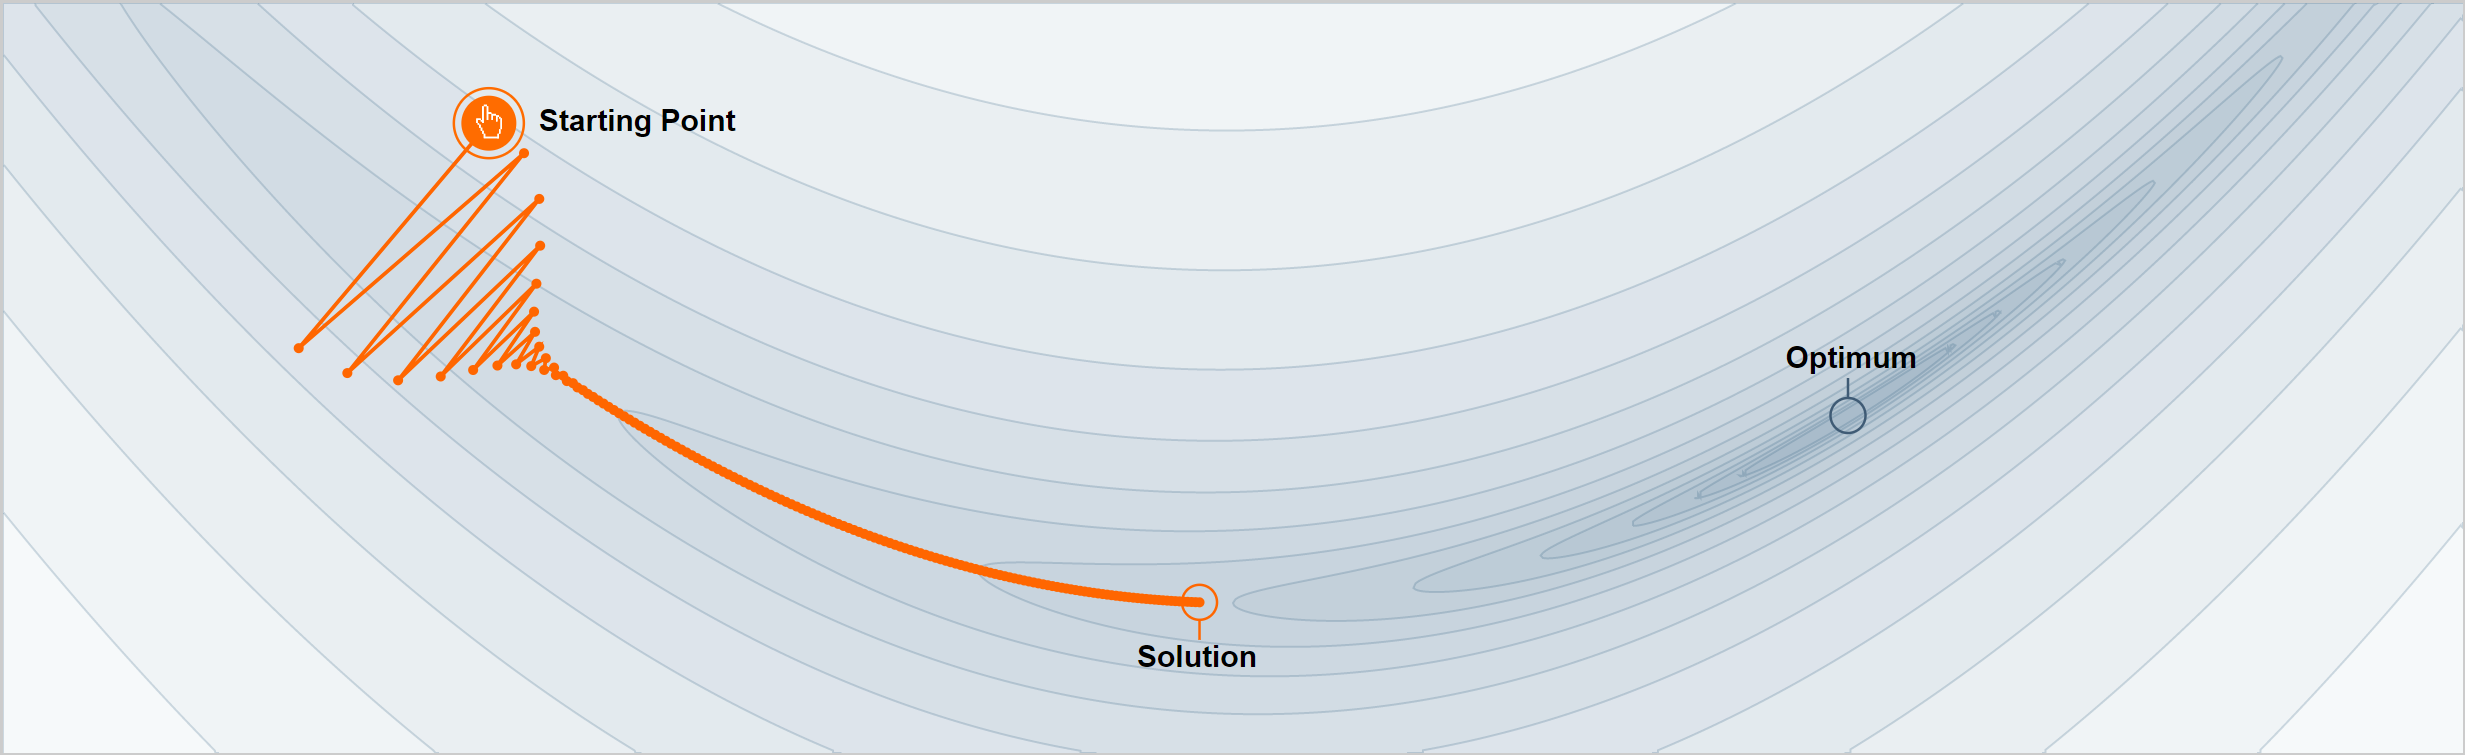
\includegraphics[width=0.7\linewidth]{06/momentum1}
        \caption{Without momentum}       
    \end{subfigure}
    \vfill
    \begin{subfigure}[b]{\linewidth}
        \centering
        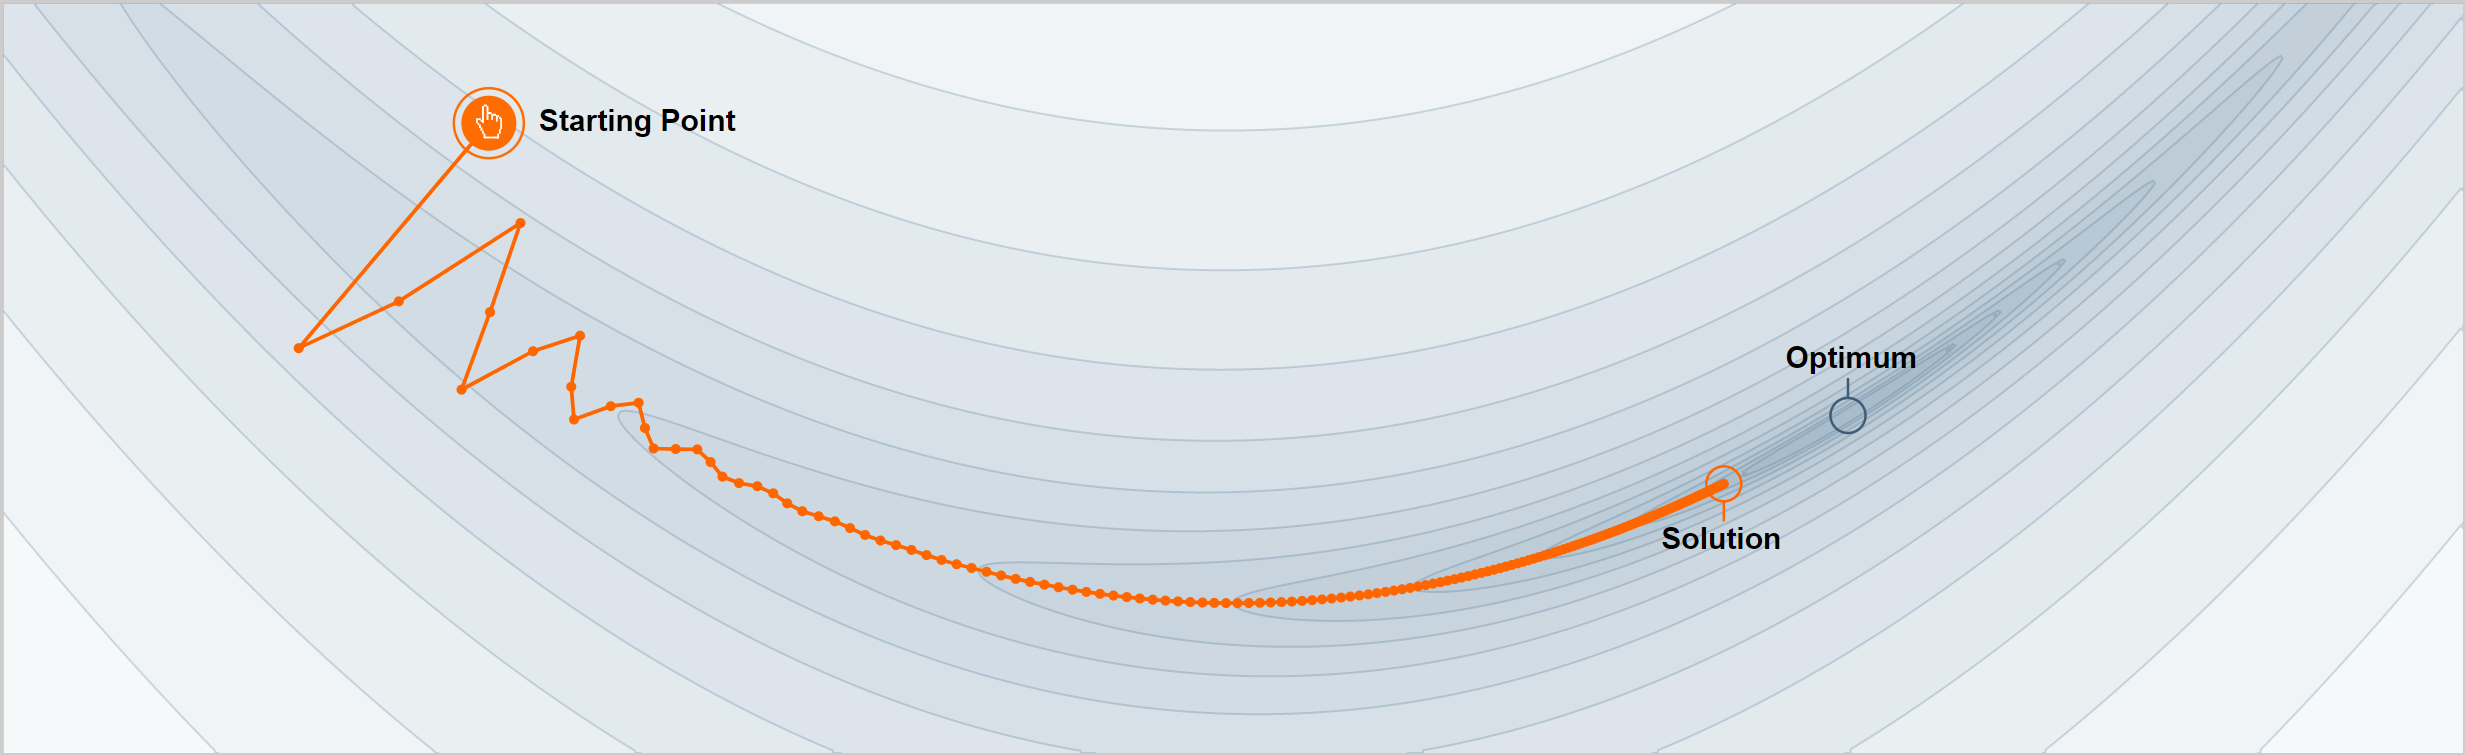
\includegraphics[width=0.7\linewidth]{06/momentum2}
        \caption{With momentum}
    \end{subfigure}
    \caption{Acceleration effect of momentum in situations with small step size.}
    \label{fig:chap6:momentum}
\end{figure}

Let's try to be more formal now. The update rule of standard gradient descent, once unrolled, has the following form:
\begin{equation}
    \begin{aligned}
        \mathbf{x}^{(1)} &= \mathbf{x}^{(0)} - \alpha \nabla f(\mathbf{x}^{(0)})  \\
        \mathbf{x}^{(2)} &= \mathbf{x}^{(1)} - \alpha \nabla f(\mathbf{x}^{(1)})  \\
        &= \mathbf{x}^{(0)}- \alpha \nabla f(\mathbf{x}^{(0)})  - \alpha \nabla f(\mathbf{x}^{(1)})  \\
        \vdots & \\
        \mathbf{x}^{(t+1)} & = \mathbf{x}^{(0)} - \alpha \sum_{i=0}^t \nabla f(\mathbf{x}^{(i)}).
    \end{aligned}
\end{equation}

Repeating the same procedure with the momentum we get
\begin{equation}
    \mathbf{x}^{(t+1)} = \mathbf{x}^{(0)} + \alpha \sum_{i=0}^t \frac{1-\lambda^{t+1-i}}{1-\lambda} \nabla f(\mathbf{x}^{(i)})
\end{equation}
in which we can explicitly see the effect of accumulating gradients. Each gradient is multiplied by a factor that is exponentially closer to zero the furthest back in the past the gradient is, since $\lambda \leq 1$.

This generalizes to the following form
\begin{equation}
    \mathbf{x}^{(t+1)} = \mathbf{x}^{(0)} + \alpha \sum_{i=0}^t \Gamma_i^{t} \nabla f(\mathbf{x}^{(i)}) \quad\textrm{for some diagonal matrix}~\Gamma_i
\end{equation}
and many optimization algorithms (ADAM, AdaGrad, etc.) derived by gradient descent, take this form, with different specific rules for the diagonal matrix, that gives more or less importance to the various components of the gradient vector in a linear and decoupled way.
